\clearpage
\subsection{For Loop} % (fold)
\label{sub:for_loop}

As has been shown in previous chapters, Computers can only perform simple actions. They cannot perform an action on all of the elements in our arrays. For example, a computer cannot sum \textbf{all} of the values in an array. What you need to do is think of these tasks so that they can be performed \textbf{for \emph{each}} value in the array. So the sum would become, for each of the numbers in the array, add the number to a running total. When this has been performed for each element in the array you have the sum of all of the elements.

The for loop is a \nameref{sub:pre_test_loop} that repeats a block of code a number of times. You can think of it like a counting loop, with it counting from a start value to an end value. The for loop has a \textbf{control variable} that has the number of the current loop as its value.

\begin{figure}[h]
   \centering
   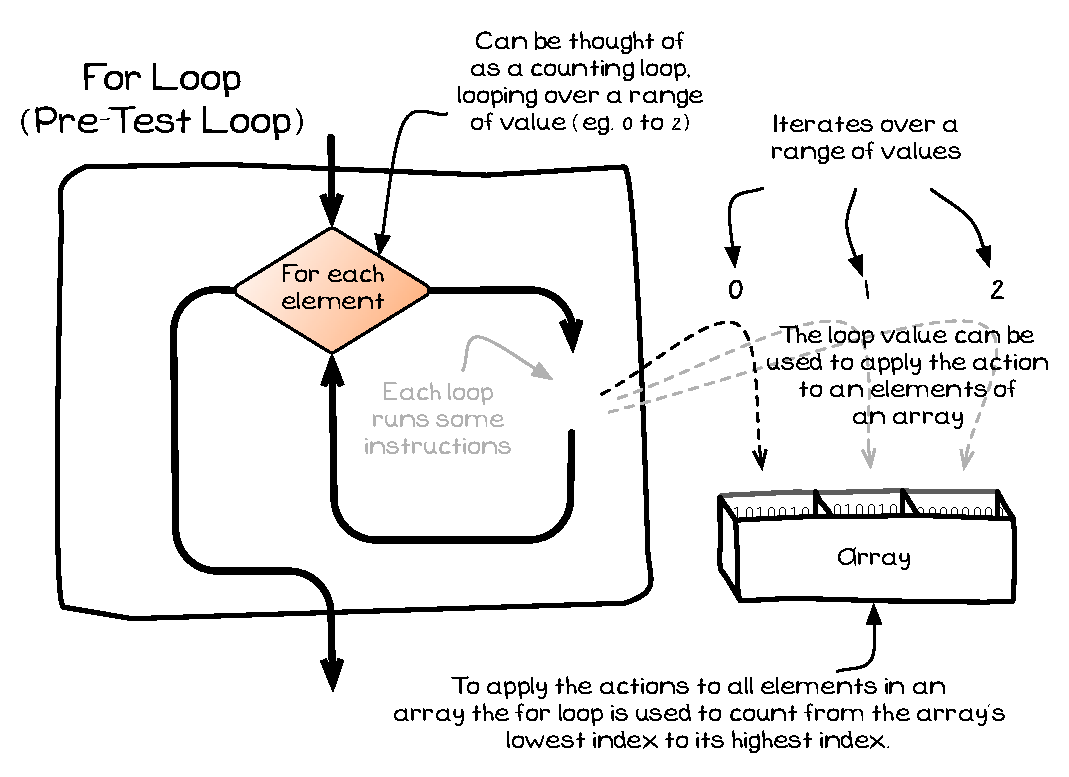
\includegraphics[width=\textwidth]{./topics/arrays/diagrams/For} 
   \caption{The for loop can be used to loop through the elements of an array}
   \label{fig:for-loop}
\end{figure}

\mynote{
\begin{itemize}
  \item A for loop is an \textbf{action}, a kind of statement you can use to command the computer to perform an action.
  \item The key is to think about processing \textbf{each} element in an array, rather than thinking about \emph{all} elements of an array.
  \item The for loop can then provide the infrastructure to repeat this code \emph{for each} element in the array.
  \item The for loop is designed to work well with the array. The values in the \emph{control variable} can be used to access the individual elements of the array.
  \item When processing the elements of an array you have it loop from the lowest index value (0) to the highest index value (n - 1).
\end{itemize}
}

% subsection for_loop (end)